\scanpage{71}
\margin{\figure{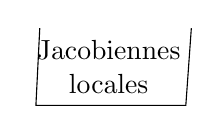
\begin{tikzpicture}[x=.7cm,y=.7cm]
\node[align=center] at (1.1,.65) {Jacobiennes\\locales};
\draw (-.15,1.35)--(-.22,-.05)--(2.5,-.05)--(2.6,1.35);
\end{tikzpicture}}}
% loop at upper left; possibly a physical paperclip
\figure{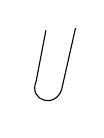
\begin{tikzpicture}[scale=.5]\draw (0,1.6)--(-.25,.3)..controls(-.45,-.2)and(.25,-.4)..(.4,.1)--(.75,1.65);\end{tikzpicture}}
\unsure{Tout dépend de quelle théorie}. \unsure{Il y en a plusieurs} :

I) Théorie \unsure{Čechiste} pour la topologie de Zariski.

(Celle où le $H^1$ \unsure{classifie} les \deleted{\unsure{ses}} fibrés principaux \uline{loc.} \uline{triviaux}). Il n'y a \inserted{\unsure{à priori}} de \unsure{suite exacte de coh.} pour $0-G'-G-G''-0$ \uline{que} si la suite est \unsure{loc triviale}.

Si $X=\unsure{\operatorname{Spec}|\operatorname{Sp}}(A)$ est le spectre d'un anneau \uline{local} on aura
\[
\begin{aligned}
H^i(X,G)&=0&&\text{si }i>0\\
H^i(X-a,G)&=0&&\text{si }i\geq\dim A\quad\deleted{\unsure{\dim(X-a)+1}}
\end{aligned}
\]
\inserted{[car $\dim(X-a)\leq\dim A-1$]}

d'où
\[
0-H^0(X/X-a,G)-H^0(X,\unsure{G})-H^0(X-a,G)-H^1(X/X-a,G)\longrightarrow0
\]
\[
H^i(X/X-a,G)\xleftarrow[\sim]{\unsure{\partial|\delta}}H^{i-1}(X-a,G)\qquad(i\unsure{\geq|>}2)
\]
\inserted{[\uline{c'est nul si $i>\dim A$\deleted{$\unsure{1}$}}]}

On supposera $A$ \uline{régulier}.
\[
\text{a)}\quad H_A^0(G)=\left\{\begin{aligned}
&G(A)=G(K)&&\text{si }\dim A=0\\
&0&&\text{si }\dim A>0
\end{aligned}\right.
\]
Le foncteur $H_A^0(G)$ est \unsure{exact} pour les suites \deleted{\unsure{split exactes}} \inserted{exactes} loc. triviales
\margin{\deleted{\illegible{3}} \deleted{(\unsure{distinguer cas $A$ abélien} \illegible{2} \unsure{et le cas $G$ affine})}}
\[
\text{b)}\quad H_A^1(G)=\left\{\begin{aligned}
&0&&\text{si }\dim A\neq1\\
&G(K)/G(A)&&\text{si }\dim A=1
\end{aligned}\right.
\]
Ce foncteur $H_A^1(G)$ est \unsure{exact} pour les suites exactes loc. triviales
% slanted
\margin{\unsure{Prouve que} si $\dim A=1$, ${\unsure{J|\mathscr J}}_{A/k}$ est \uline{connexe} \unsure{sans composante abélienne} (car $H_A^1(G)$ est nul pour $G$ \unsure{propre ou} $G$ discret)}
\margin{\deleted{$\unsure{G_{\mathrm{Ab}}}$}\deleted{\illegible{3}}}
\[
\text{c)}\quad H_A^2(G)=H^1(X-a,G)=\left\{\begin{aligned}
&0\text{ si }\dim A\neq2\\
&\text{\unsure{en tous cas ne dépend que de}}\\
&\text{\unsure{la composante connexe}}\\
&\text{\unsure{unipotente} de }G.
\end{aligned}\right.
\]
% archive sheet number: 70
